\section{Auswertung}
\label{sec:Auswertung}
\begin{figure}
  \centering
  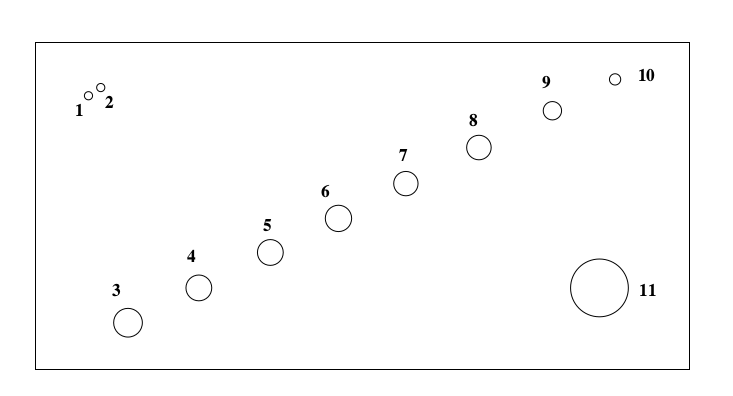
\includegraphics[width=0.8\textwidth]{Bilder/fehlstellen.png}
  \caption{Schematische Darstellung des untersuchten Acrylblocks samt der durchnummerierten Fehlstellen. \cite{Anleitung}.}
  \label{fig:fehlstellen}
\end{figure}
Zunächst werden die Durchmesser $d_\mathrm{SL}$ sämtlicher Fehlstellen mittels einer Schiebelehre ausgemessen. Die Nummerierung $n$ der Fehlstellen erfolgt nach dem Schema in Abbildung \ref{fig:fehlstellen}. Die bestimmten Durchmesser finden sich in Tabelle \ref{tab:fehlstellen}.
\begin{table}
  \centering
	\caption{Durchmesser der Fehlstellen vermessen mittels Schieblehre.}
	\label{tab:fehlstellen}
	\begin{tabular}{cc}
		\toprule
    $n$ & $d_\mathrm{SL}$/$\si{\milli\meter}$ \\
		\midrule
1.0 & 1.3 \\
2.0 & 1.3 \\
3.0 & 5.8 \\
4.0 & 4.8 \\
5.0 & 4.0 \\
6.0 & 2.9 \\
7.0 & 2.9 \\
8.0 & 2.9 \\
9.0 & 2.9 \\
10.0 & 2.9 \\
11.0 & 9.5 \\
\bottomrule
\end{tabular}
\end{table}
Zusätzlich wurde der gesamte Acrylblock mittels der Schiebelehre vermessen. Es ergibt sich eine Breite von ${\SI{8}{\centi\meter}}$. Mit der Schallgeschwindigkeit ${c=\SI{2730}{\meter\per\second}}$ nach \cite{schall} und Formel \eqref{eqn:laufzeit} ergibt sich die Laufzeit des Ultraschallsignals durch den Acrylblock zu ${t_{\mathrm{theo}}=\SI{58.6}{\micro\second}}$.
Wird allerdings die tatsächliche Laufzeit des Ultraschallsignals in der Messung bestimmt, ergibt sich eine Laufzeit von ${t_\mathrm{real}=\SI{60.6}{\micro\second}}$. Dies liegt an der Anpassungsschicht zwischen der Ultraschallsonde und dem Acrylblock. Um in den weiteren Messungen die tatsächlichen Laufzeiten im Acrylblock zu bestimmen, muss von jedem bestimmten Wert daher die Laufzeit durch die Anpassungsschicht ${\Delta t=\SI{2}{\micro\second}}$ abgezogen werden.

%%%%%%%%%%%%%%%%%%%%%%%%%A-Scan%%%%%%%%%%%%%%%%%%%%%%%%%%%%%%%%%%%%%%%%%%%%%%%%%%%%%%%%%%%
\FloatBarrier
\subsection{Bestimmung der Abmessung der Fehlstellen über den A-Scan}
Die Messwerte zur Bestimmung der Lage der Fehlstellen sind in Tabelle \ref{tab:ascan}
aufgetragen. Hierbei wird die Lage der Fehlstelle im Acrylblock mit den gemessenen Laufzeiten
und Formel \eqref{eqn:laufzeit} bestimmt. Für die Schallgeschwindigkeit in Acryl wird der
Wert $c = \SI{2730}{\meter\per\second}$ verwendet. Weiterhin wird jeweils die Laufzeitkorrektur
von $\SI{2}{\micro\second}$ beachtet.
Die Werte $t_1$ und $s_1$ gehören zur Messung mit der Ausrichtung wie in Abbildung
\ref{fig:fehlstellen} und $t_2$ und $s_2$ gehören entsprechend zur Messung mit dem gedrehten
Acrylblock.
\begin{table}
  \centering
	\caption{Messwerte der Laufzeiten mit der Lage der zugehörigen Fehlstelle nach Formel \eqref{eqn:laufzeit} bei der normalen Ausrichtung und dem gedrehten Block.}
	\label{tab:ascan}
	\begin{tabular}{ccccc}
		\toprule
		$n$ & $t_1$/$\si{\micro\second}$ & $s_1$/$\si{\milli\meter}$ & $t_2$/$\si{\micro\second}$ & $s_2$/$\si{\milli\meter}$ \\
		\midrule
		1 & 13.8 & 18.84 & 46.3 & 63.20 \\
		2 & 16.0 & 21.84 & 43.6 & 59.51 \\
		3 & 44.3 & 60.47 & 9.9 & 13.51 \\
		4 & 39.3 & 53.64 & 15.9 & 21.70 \\
		5 & 33.8 & 46.14 & 22.2 & 30.30 \\
		6 & 28.4 & 38.77 & 28.2 & 38.49 \\
		7 & 22.7 & 30.99 & 34.2 & 46.68 \\
		8 & 17.0 & 23.21 & 40.0 & 54.60 \\
		9 & 11.0 & 15.02 & 45.8 & 62.52 \\
		10 & 5.2 & 7.10 & 51.9 & 70.84 \\
		11 & 40.6 & 55.42 & 11.2 & 15.29 \\
		\bottomrule
	\end{tabular}
\end{table}
Aus den Positionen der Hin- und Rückseite der jeweiligen Fehlstellen lässt sich nun der
Durchmesser der Fehlstellen durch
\begin{equation*}
	d = \SI{8}{\centi\meter} - s_1 - s_2
\end{equation*}
berechnen.
Die so bestimmten Durchmesser der Fehlstellen sind in Tabelle \ref{tab:durchfehl} zu finden.
\begin{table}
  \centering
	\caption{Berechneten Durchmesser der Fehlstellen im Acrylblock.}
	\label{tab:durchfehl}
	\begin{tabular}{cc}
		\toprule
		$n$ & $d$/$\si{\milli\meter}$ \\
		\midrule
		1 & 2.0 \\
		2 & 1.4 \\
		3 & 6.0 \\
		4 & 4.7 \\
		5 & 3.6 \\
		6 & 2.7 \\
		7 & 2.3 \\
		8 & 2.2 \\
		9 & 2.6 \\
		10 & 2.1 \\
		11 & 9.3 \\
		\bottomrule
	\end{tabular}
\end{table}

%%%%%%%%%%%%%%%%%%%%%%%%%%%%%%%Axiale Aufösung%%%%%%%%%%%%%%%%%%%%%%%%%%%%%%%%%%%%%%%%%
\FloatBarrier
\subsection{Untersuchung des Auflösungsvermögen}
Zur Untersuchung des Auflösungsvermögen werden die Fehlstellen 1 und 2 aus Abbildung
\ref{fig:fehlstellen} betrachtet.
Bei einem A-Scan mit einer $\SI{4}{\mega\hertz}$ Sonde wurden die beiden Laufzeiten bei
Reflexionen an der Hinseite der Fehlstellen 1 und 2 zu
\begin{align*}
	t_1 &= \SI{13.6}{\micro\second} \, \mathrm{,} \\
	t_2 &= \SI{14.8}{\micro\second} \, \mathrm{.}
\end{align*}
Damit ergeben sich mit Formel \eqref{eqn:laufzeit} die beiden Lagen der Fehlstellen zu
\begin{align*}
	s_1 &= \SI{18.6}{\milli\meter} \, \mathrm{,} \\
	s_2 &= \SI{20.2}{\milli\meter} \, \mathrm{.}
\end{align*}
Da die $\SI{4}{\mega\hertz}$ Sonde durch die höhere Frequenz eine geringere Eindringtiefe
hat, wird die Lage der Rückseite aus Tabelle \ref{tab:ascan} verwendet.
Es ergeben sich die beiden Dicken der Fehlstellen 1 und 2 zu
\begin{align*}
	d_1 &= \SI{1.8}{\milli\meter} \, \mathrm{,} \\
	d_2 &= \SI{0.3}{\milli\meter} \, \mathrm{.}
\end{align*}
Es lässt sich also sagen, dass eine höhere Frequenz durch die kleinere Wellenlänge
für eine bessere Auflösung sorgt.
Allerdings folgt aus einer höheren Frequenz auch eine geringere Eindringtiefe, sodass die
Reflexionen an der Hin- und Rückseite der Fehlstelle an dem näheren Ende des Acrylblocks zu
erkennen sein müssen.
Da die Reflexion an der hinteren Seite der Fehlstelle nicht zu erkennen war, muss also für
einen Vergleichswert die Laufzeit für die Reflexion mit der $\SI{1}{\mega\hertz}$ Sonde
verwendet werden, was bei der zweiten Fehlstelle sogar für eine größere Abweichung vom gemessenen
Durchmesser sorgt. Der erste Durchmesser hingegen liegt näher am erwarteten Wert.

%%%%%%%%%%%%%%%%%%%%%%BScan%%%%%%%%%%%%%%%%%%%%%%%%%%%%%%%%%%%%%%%%%%%%%%%%%%%%%%%%%%%%%%
\subsection{Bestimmung der Abmessung der Fehlstellen über den B-Scan}
\label{sec:bscan}
\begin{figure}
  \centering
  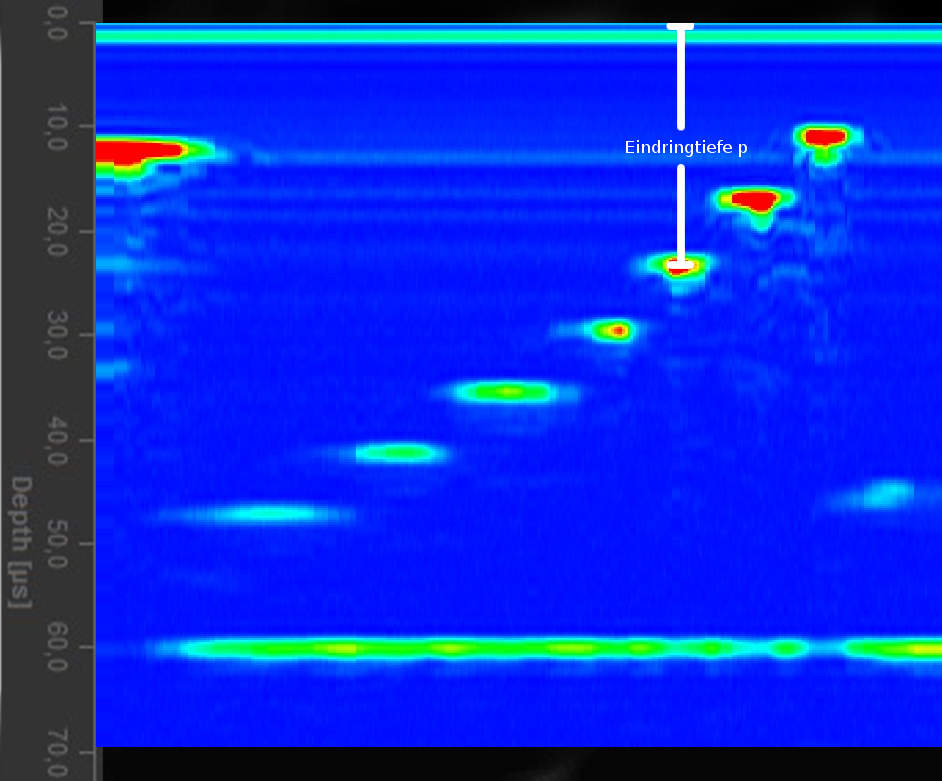
\includegraphics[width=0.72\textwidth]{bscan/messverfahren}
  \caption{Darstellung zur Verdeutlichung des verwendeten Skalierungsverfahren.}
  \label{fig:messverfahren}
\end{figure}
Zur Bestimmung der Abmessung der Fehlstellen über den B-Scan wird der Abstand $p$ jeder Fehlstelle mittels des freien Grafikprogramms \enquote{Gimp} in Pixeln bezüglich der oberen Bildkante bestimmt (vgl. dazu Abbildung \ref{fig:messverfahren}).
Diese Skalierung kann umgerechnet werden auf die Eindringtiefe $s_\mathrm{msec}$ in Microsekunden, da bekannt ist, dass die Bildhöhe von $h=\num{724}$ Pixeln einer Eindringtiefe von $\SI{69}{\micro\second}$ entspricht.
Es ergibt sich die Umrechnung:
\begin{equation}
  s_\mathrm{sec}=\frac{69\, \si{\micro\second}}{724}\cdot p \text{.}
\end{equation}
Zusätzlich wird, wie zu Beginn der Auswertung erläutert, von jedem so ermittelten Wert die Anpassungsschicht abgezogen. Diese wird graphisch bestimmt zu $t=\SI{0.9}{\micro\second}$.
In Tabelle \ref{tab:bscan} finden sich die so berechneten Eindringtiefen in Microsekunden $s_\mathrm{sec}$ sowie die hieraus nach Formel \eqref{eqn:laufzeit} berechneten Eindringtiefen in Millimetern $s_\mathrm{mm}$.\\
Die Schallgeschwindigkeit in Acryl ist $c_\mathrm{Acryl}=\SI{2730}{\meter\per\second}$.\\
Hierbei bezeichnet $s_\mathrm{h,sec}$ und $s_\mathrm{h,mm}$ den Scan der Oberseite (vgl. dazu Abbildung \ref{fig:b1} ) und $s_\mathrm{r,sec}$ sowie $s_\mathrm{r,mm}$ den Scan der Unterseite (siehe Abbildung \ref{fig:b2}).
In der sechsten Spalte findet sich schließlich der mittels B-Scan bestimmte Durchmesser $d_\mathrm{B}$ der Fehlstellen. Außerdem wird der experimentell bestimmte Durchmesser verglichen mit dem mittels Schieblehre ermittelten Durchmesser $d_\mathrm{SL}$ der Fehlstellen.
Einige Fehlstellen konnten nicht aus den Plots abgelesen werden und sind daher nicht angegeben.
\begin{figure}
  \centering
  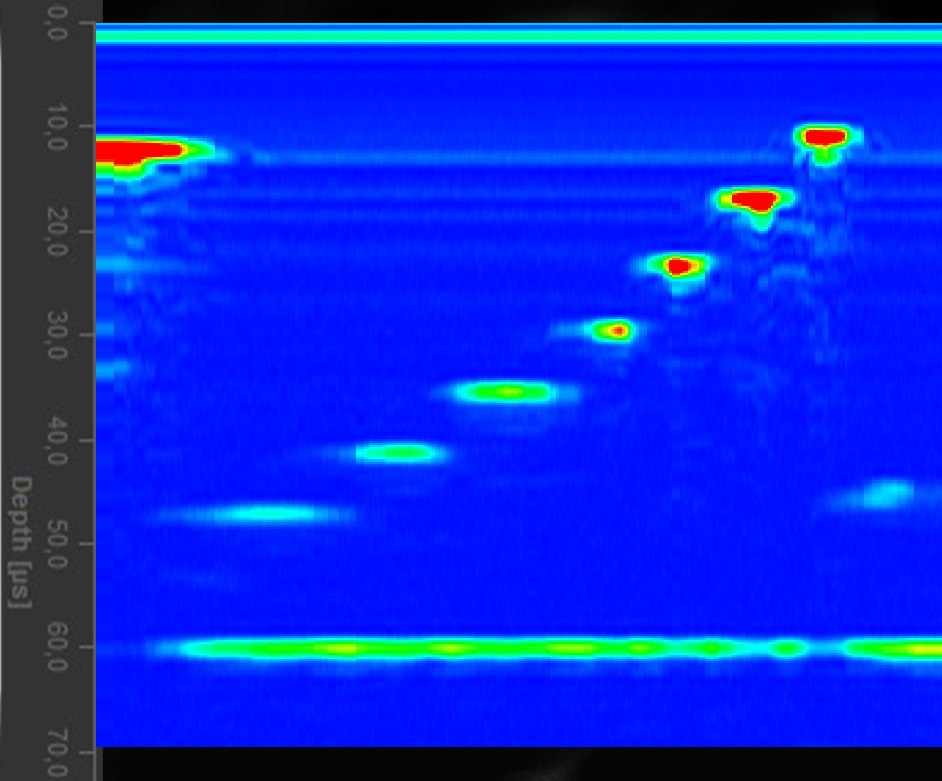
\includegraphics[width=0.7\textwidth]{bscan/bscan2rueck}
  \caption{B-Scan des Acrylblocks zur Bestimmung der Abmessung der Fehlstellen (Unterseite).}
  \label{fig:b2}
\end{figure}

\begin{figure}
  \centering
  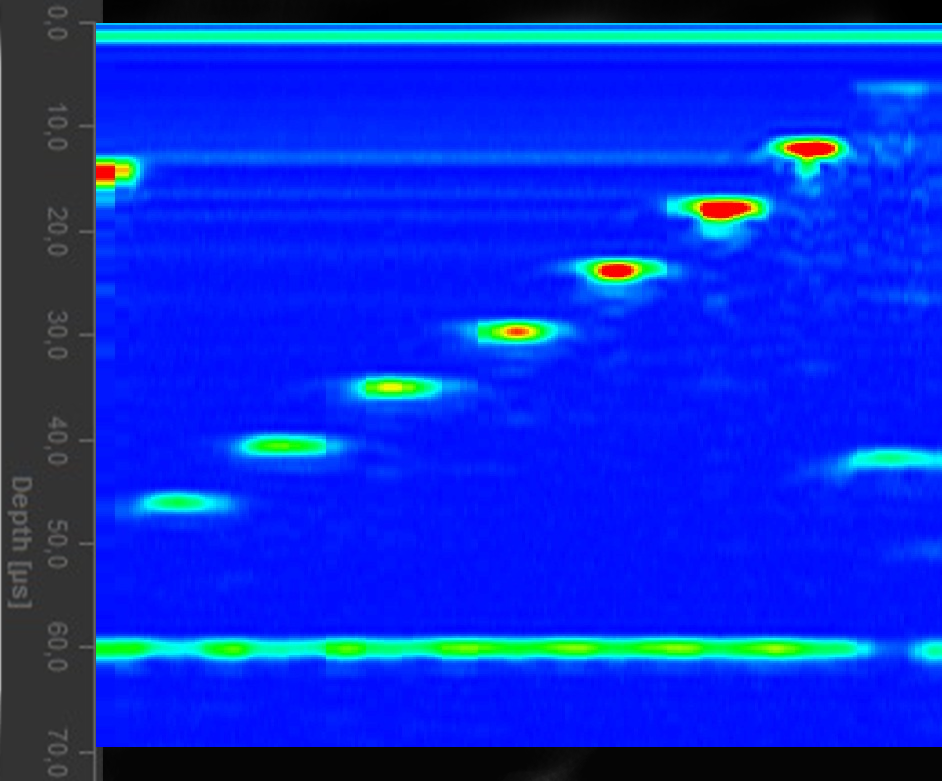
\includegraphics[width=0.7\textwidth]{bscan/bscan2}
  \caption{B-Scan des Acrylblocks zur Bestimmung der Abmessung der Fehlstellen (Oberseite).}
  \label{fig:b1}
\end{figure}

\begin{table}
  \centering
  \caption{Bestimmung der Abmessung der Fehlstellen anhand des B-Scans.}
  \label{tab:bscan}
\begin{tabular}{cccccccc}
\toprule
$n$ & $s_\mathrm{h,sec}$/$\si{\micro\second}$ &$s_\mathrm{r,sec}$/$\si{\micro\second}$  & $s_\mathrm{h,mm}$/$\si{\centi\meter}$  & $s_\mathrm{r,mm}$/$\si{\centi\meter}$& $d_\mathrm{B}$/$\si{\centi\meter}$& $d_\mathrm{SL}$/$\si{\centi\meter}$ & $\Delta d$ in $ \%$ \\
\midrule
1.0 & -- & 43.6 & -- & 5.95 & -- & 0.13 & -- \\
2.0 & 12.8 & 44.7 & 1.75 & 6.1 & 0.15 & 0.13 & 15.4 \\
3.0 & 44.8 & 10.0 & 6.11 & 1.36 & 0.53 & 0.58 & 8.6 \\
4.0 & 39.2 & 16.0 & 5.35 & 2.18 & 0.47 & 0.48 & 2.1 \\
5.0 & 33.6 & 22.3 & 4.59 & 3.04 & 0.38 & 0.4 & 5.0 \\
6.0 & 28.3 & 28.5 & 3.86 & 3.88 & 0.26 & 0.29 & 10.3 \\
7.0 & 22.5 & 34.4 & 3.08 & 4.69 & 0.23 & 0.29 & 20.7 \\
8.0 & 16.5 & 40.2 & 2.26 & 5.48 & 0.26 & 0.29 & 10.3 \\
9.0 & 10.8 & 46.0 & 1.48 & 6.28 & 0.25 & 0.29 & 13.8 \\
10.0 & 5.0 & -- & 0.68 & -- & -- & 0.29 & -- \\
11.0 & 40.5 & 11.2 & 5.52 & 1.53 & 0.95 & 0.95 & 0 \\
\bottomrule
\end{tabular}
\end{table}
\FloatBarrier
\subsection{Untersuchung eines Herzmodells mit dem TM-Scan}
Das Herz arbeitet in einem wellenartigen Pumpvorgang. Grundlegend kann zwischen zwei Phasen unterschieden werden. Einmal der diastolischen Phase, in dieser ist der Herzmuskel entspannt und das Herz füllt sich mit Blut und erreicht sein maximales Volumen (enddiastolisches Volumen EDV); anschließend tritt die systolische Phase auf; das Herz zieht sich zusammen und das zuvor in ihm befindliche Blut wird in den Lungenkreislauf beziehungsweise in den Körperkreislauf gepumpt. Das Herz erreicht schließlich sein kleinstes, das sogenannte endsystolische Volumen (ESV).\\
Das sogenannte Herzzeitvolumen (HZV) bezeichnet die pro Zeiteinheit durch das Herz gepumpte Blutmenge und wird berechnet über die Herzfrequenz  und der Herzvoluminadifferenz zwischen Systole und Diastole:
\begin{equation}
  HZV=\left(EDS-EDV\right)\cdot \nu_\mathrm{Herz} \text{.}
\end{equation}

Aus dem TM-Scan des schlagenden Herzens (vgl. Abbildung \ref{fig:herz}) lässt sich die Herzfrequenz über die Anzahl der Maxima $n=13$ und die Laufzeit des TM-Scan $\Delta t=\SI{10}{\second}$ bestimmt zu
\begin{equation*}
  \nu_\mathrm{Herz}=\frac{13}{10}=\SI{1.3}{\Hz} \text{.}
\end{equation*}

\begin{figure}
  \centering
  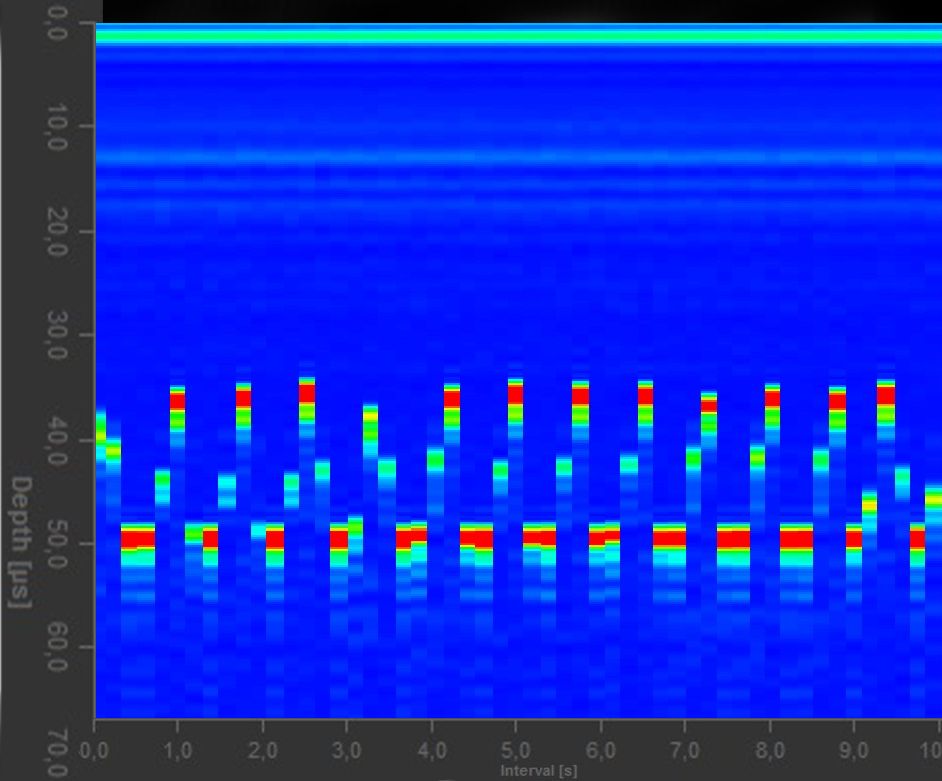
\includegraphics[width=0.75\textwidth]{bscan/herz1}
  \caption{TM-Scan des pumpenden Herzmodell.}
  \label{fig:herz}
\end{figure}

Aus dem TM-Scan lässt sich zudem nach der selben Methode wie in Abschnitt \ref{sec:bscan} die jeweilige Eindringtiefe des Ultraschalls bestimmen.
Die Umrechnung ergibt sich hier zu
\begin{equation}
  s_\mathrm{sec}=\frac{69\, \si{\micro\second}}{706}\cdot p \text{.}
\end{equation}
\begin{table}
  \centering
  \caption{TM-Scan des pumpenden Herzens zur Bestimmung des Herzzeitvolumens.}
  \label{tab:herz}
\begin{tabular}{ccccc}
  \toprule
$n$& $s_\mathrm{min,sec}$/$\si{\micro\second}$ &$s_\mathrm{max,sec}$/$\si{\micro\second}$  & $s_\mathrm{min,mm}$/$\si{\centi\meter}$  & $s_\mathrm{max,mm}$/$\si{\centi\meter}$ \\
\midrule
1  & 50.14 & 39.88 & 3.75 & 2.98 \\
2  & 50.63 & 36.94 & 3.79 & 2.77 \\
3  & 50.24 & 36.85 & 3.76 & 2.76 \\
4  & 50.43 & 36.06 & 3.77 & 2.7 \\
5  & 50.04 & 38.31 & 3.75 & 2.87 \\
6  & 50.14 & 36.55 & 3.75 & 2.74 \\
7  & 50.14 & 36.16 & 3.75 & 2.71 \\
8  & 49.94 & 36.45 & 3.74 & 2.73 \\
9  & 50.14 & 36.55 & 3.75 & 2.74 \\
10  & 50.43 & 37.63 & 3.77 & 2.82 \\
11  & 50.33 & 36.75 & 3.77 & 2.75 \\
12  & 50.14 & 36.85 & 3.75 & 2.76 \\
13  & 50.53 & 36.55 & 3.78 & 2.74 \\
\bottomrule
\end{tabular}
\end{table}

In Tabelle \ref{tab:herz} finden sich die mittels Umrechnung bestimmten Eindringtiefen für alle Minima $s_\mathrm{t,min}$ und Maxima $s_\mathrm{t,max}$, sowie die daraus berechneten Eindringtiefen in Millimetern.\\
Die hierfür verwendete Schallgeschwindigkeit in bidestillierten Wasser beträgt $c=\SI{1497}{\meter\per\second}$ nach \cite{schall}.
Das enddiastolische Volumen ($EDV$) entspricht einem Zylinder mit Höhe $h_\mathrm{dia}=\overline{s}_\mathrm{mm,min}$ und Radius $r=\SI{6}{\centi\meter}$.
Das endsystolische Volumen errechnet sich aus dem Zylinder des enddiastolischen Volumens abzüglich des durch die gewölbte Gummimembran gebildete Kugelsegments. Das Volumen eines Kugelsegments errechnet sich über
\begin{equation}
  V=\frac{\pi}{3}h^2\left (3 \cdot r - h\right)
\end{equation}
nach \cite{bronstein}.
Der Radius $r=\SI{6}{\centi\meter}$ entspricht hier dem Radius des Gummimembran des Herzmodells und die Höhe des Kugelsegments berechnet sich über:
\begin{equation*}
  h=h_\mathrm{dia}-h_\mathrm{sys}=\overline{s}_\mathrm{mm,min}-\overline{s}_\mathrm{mm,max}=\SI{3.76}{\centi\meter}-\SI{2.77}{\centi\meter}=\SI{0.99}{\centi\meter}
\text{.}
\end{equation*}
Damit gilt für das Schlagvolumen:
\begin{equation*}
  V_\mathrm{Schlag}=EDS-EDV=\SI{17.41}{\cubic\centi\meter}\text{,}
\end{equation*}
das Herzzeitvolumen ergibt sich daher zu:
\begin{equation*}
  HZV=\left(EDS-EDV\right)\cdot \nu_\mathrm{Herz}=\left(\frac{\pi}{3}h^2\left (3 \cdot r - h\right) \right) \nu_\mathrm{Herz}=\SI{22.638}{\cubic\centi\meter\per\second}\text{.}
\end{equation*}


%%Vorlagen
%Bild
%\begin{figure}
%  \centering
%  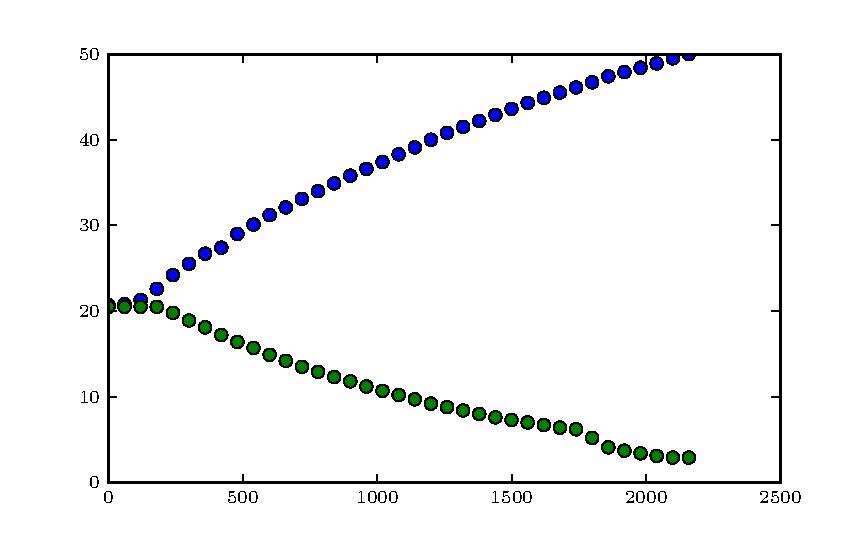
\includegraphics{plot.pdf}
%  \caption{Plot.}
%  \label{fig:plot}
%\end{figure}


%Tabelle
%\begin{table}
%	\centering
%	\caption{Table.}
%	\label{tab:table}
%	\begin{tabular}{ccc}
%		\toprule
%    column1&column2&column3\\
%		\midrule
%		220 & -391 & 659 \\
%		330 & -598 & 946 \\
%		525 & -1000 & 1660 \\
%		702 & -1337 & 2051 \\
%		930 & -1650 & 2450 \\
%		\bottomrule
%	\end{tabular}
%\end{table}
